\chapter{Experimental Results}

\section{Cross distance histogram}

\subsection{Small translations} \label{sec:relief_small_trans_exp}
The following figures depict cross distance histograms of a relief point cloud $P$ like the one on figure \ref {fig:relief_plain}, on which a small transformation $\matr{M}$ was applied. For the point cloud $P$, the average nearest neighbor distance on surfaces perpendicular to the camera ray is $p_l = 0.01$. The plane of the relief is along the X and Y axis.


\subsubsection{Translation in X and Y axis}
$\matr{M}$ is a translation in X and Y axis, by the amounts \{ 0, 0.001, 0.003, 0.009, 0.027, 0.081 \}. No translation in Z axis and no rotation is applied.

The top-left cell shows the own distance histogram, where $\matr{M} = \matr{I}$. Only translations in the positive directions are made, translations in the negative directions would yield similar results.

\begin{figure}[H]
\foreach \y in {0,1,2,3,4} {
	\foreach \x in {0,1,2,3,4} {
		\includegraphics[width=0.19\linewidth]{fig/cross_relief_trans/(\x-\y-0).pdf}
	}
	\\
}
\caption{Horizontal: X translation, vertical: Y translation}
\end{figure}

\subsubsection{Translation in X and Z axis}
Y axis translation fixed to $0$. Translations by same amounts.

\begin{figure}[H]
\foreach \z in {0,1,2,3,4} {
	\foreach \x in {0,1,2,3,4} {
		\includegraphics[width=0.19\linewidth]{fig/cross_relief_trans/(\x-0-\z).pdf}
	}
	\\
}
\caption{Horizontal: X translation, vertical: Z translation}
\end{figure}


\subsection{Small rotations}
Here instead of a translation, a rotation gets applied on the same point cloud. The point of rotation is the center point of the relief plane. The amounts of rotation are \{ 0, 0.001\si{\degree}, 0.003\si{\degree}, 0.009\si{\degree}, 0.027\si{\degree}, 0.081\si{\degree} \}.

\subsubsection{Rotation around X and Y axis}
\begin{figure}[H]
\foreach \y in {0,1,2,3,4} {
	\foreach \x in {0,1,2,3,4} {
		\includegraphics[width=0.19\linewidth]{fig/cross_relief_rot/(\x-\y-0).pdf}
	}
	\\
}
\caption{Horizontal: X axis rotation, vertical: Y axis rotation}
\end{figure}


\subsubsection{Rotation around X and Z axis}
\begin{figure}[H]
\foreach \z in {0,1,2,3,4} {
	\foreach \x in {0,1,2,3,4} {
		\includegraphics[width=0.19\linewidth]{fig/cross_relief_rot/(\x-0-\z).pdf}
	}
	\\
}
\caption{Horizontal: X axis rotation, vertical: Z axis rotation}
\end{figure}



\section{Different resolutions, Bunny model}
\begin{tabularx}{\textwidth}{|r|X|} \hline
Method & ICP. Select all points, closest point criterion, equal weights, no rejection, point-to-point error metric. \\ \hline
Model & Stanford Bunny model. \\ \hline
Fixed & 50\% of model points, randomly chosen. \\ \hline
Loose & Starting from the other 50\%, randomly downsampled by given amount. $60$ steps. \\ \hline
Displacement & See captions on the figures. \\ \hline
Y Axis & True error, after $40$ iterations. \\\hline
X Axis & Number of points in Loose divided by number of points in Fixed. \\ \hline
\end{tabularx}


\subsection{Final true error v. downsampling level} \label{sec:bunny_hilo}

\begin{figure}[H]
\centering
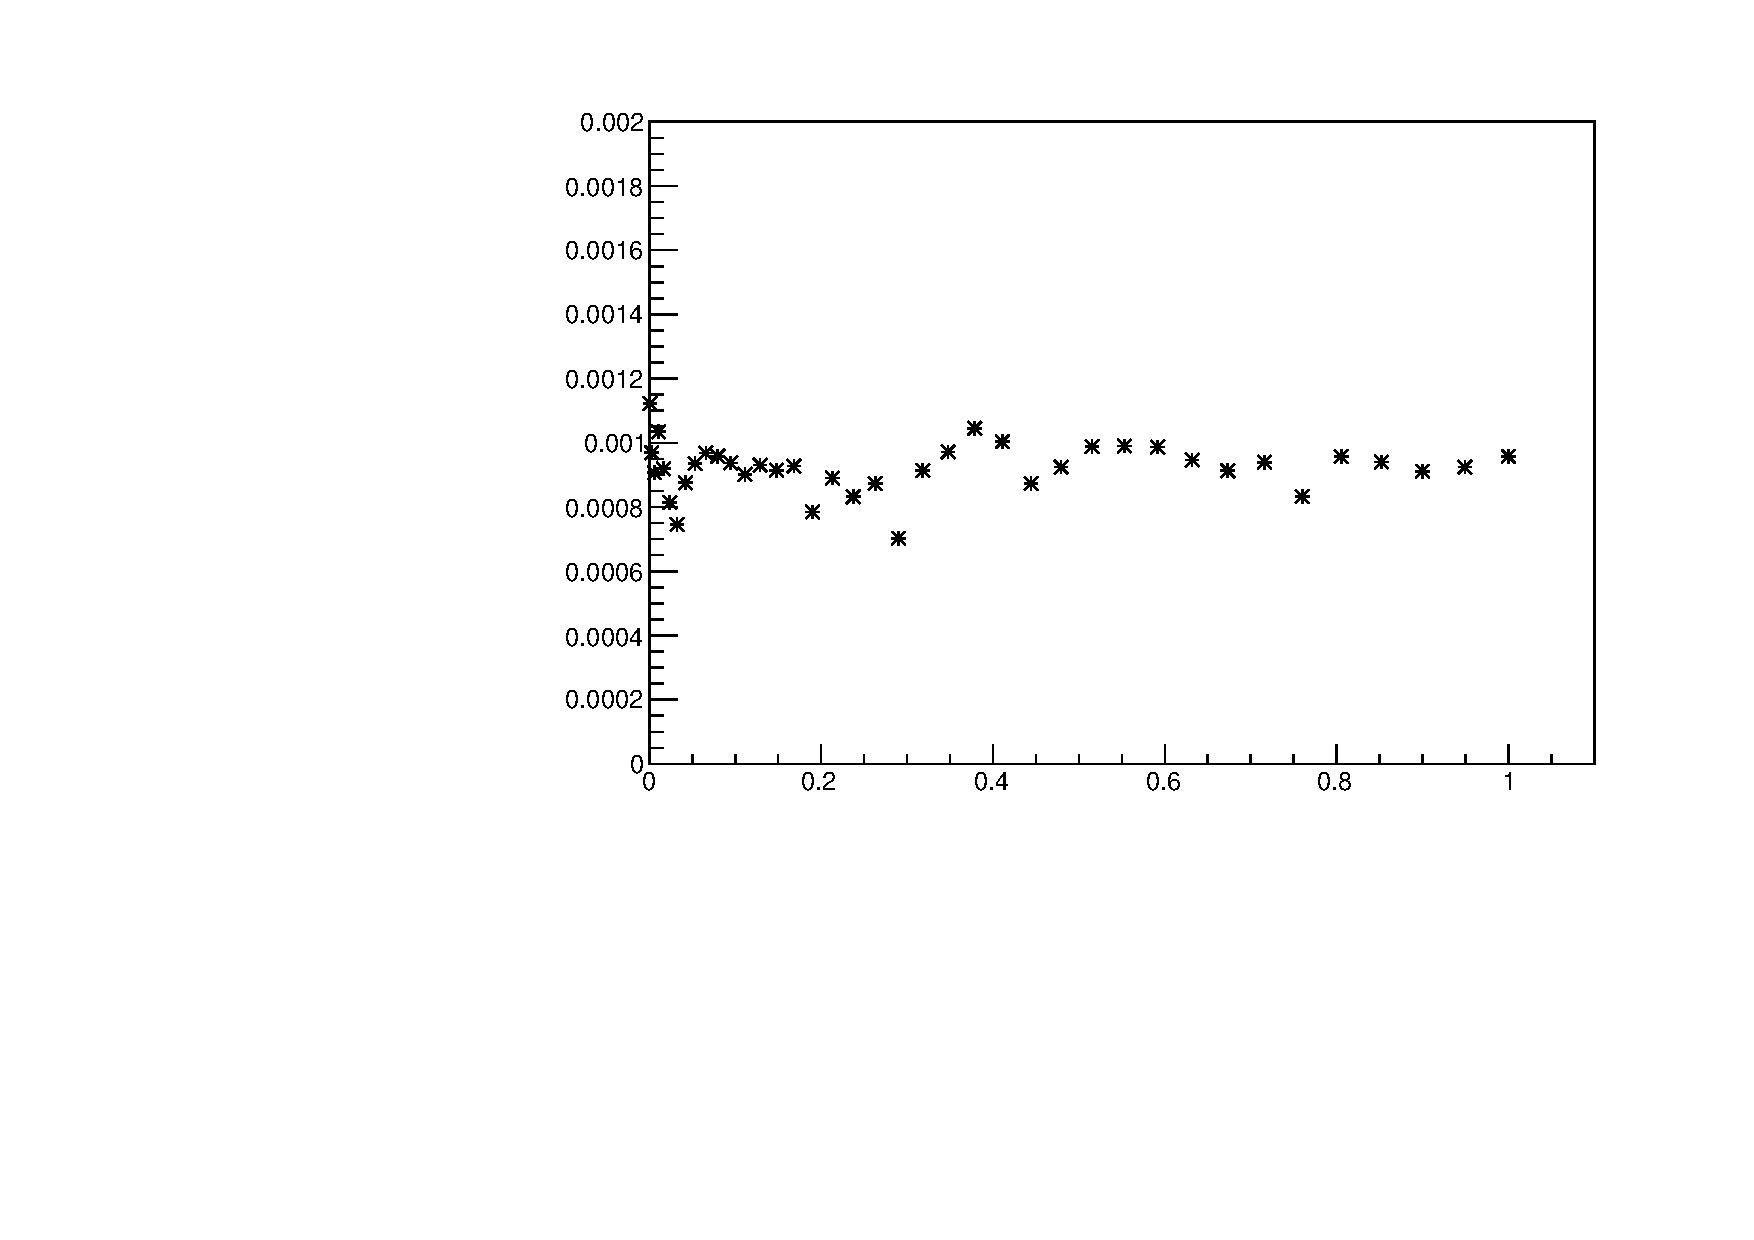
\includegraphics[width=.7\textwidth]{fig/bunny_globmin.pdf}
\caption{no displacement}
\label{fig:bunny_globmin}
\end{figure}
\begin{figure}[H]
\centering
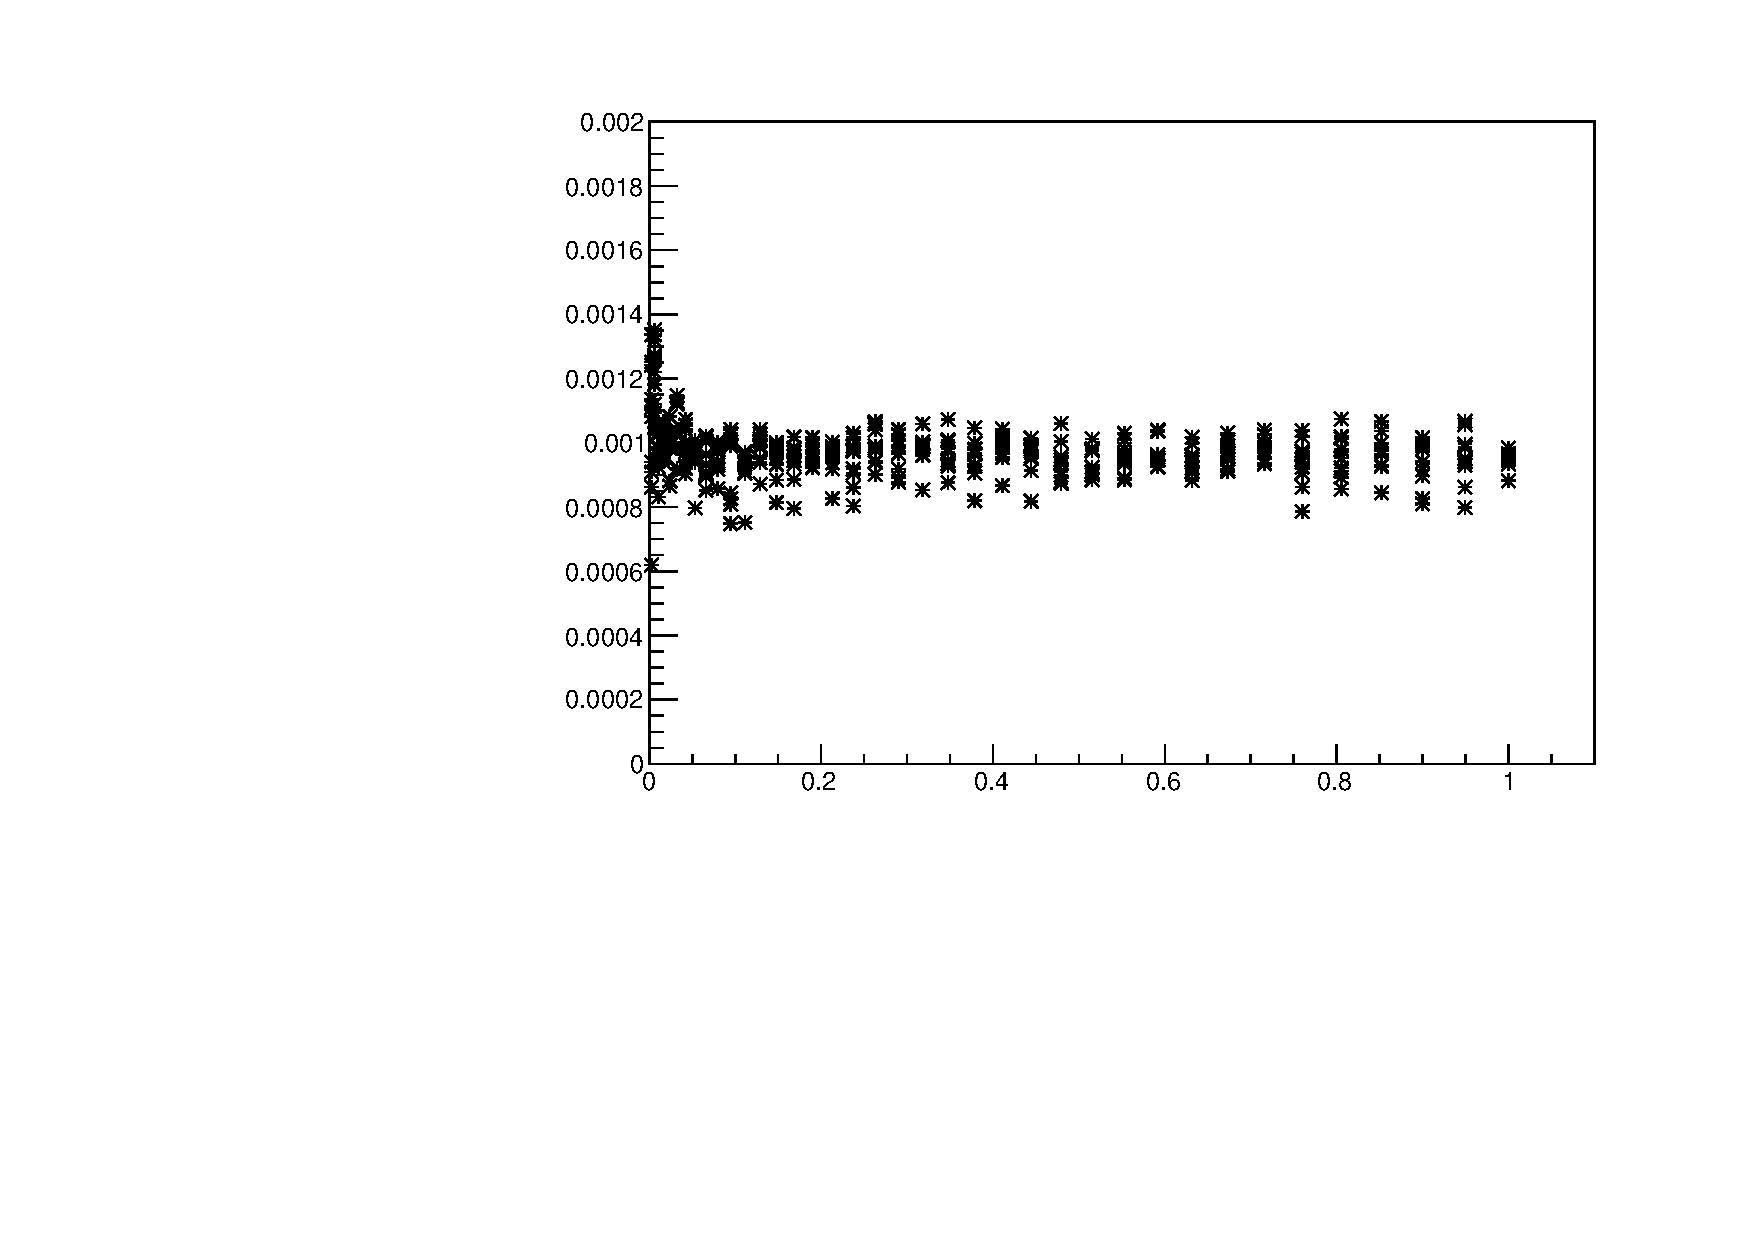
\includegraphics[width=.7\textwidth]{fig/bunny_globsmall.pdf}
\caption{random translation of $0.01$ and rotation of $3 \si{\degree}$, chosen $10$ times}
\label{fig:bunny_globsmall}
\end{figure}
\begin{figure}[H]
\centering
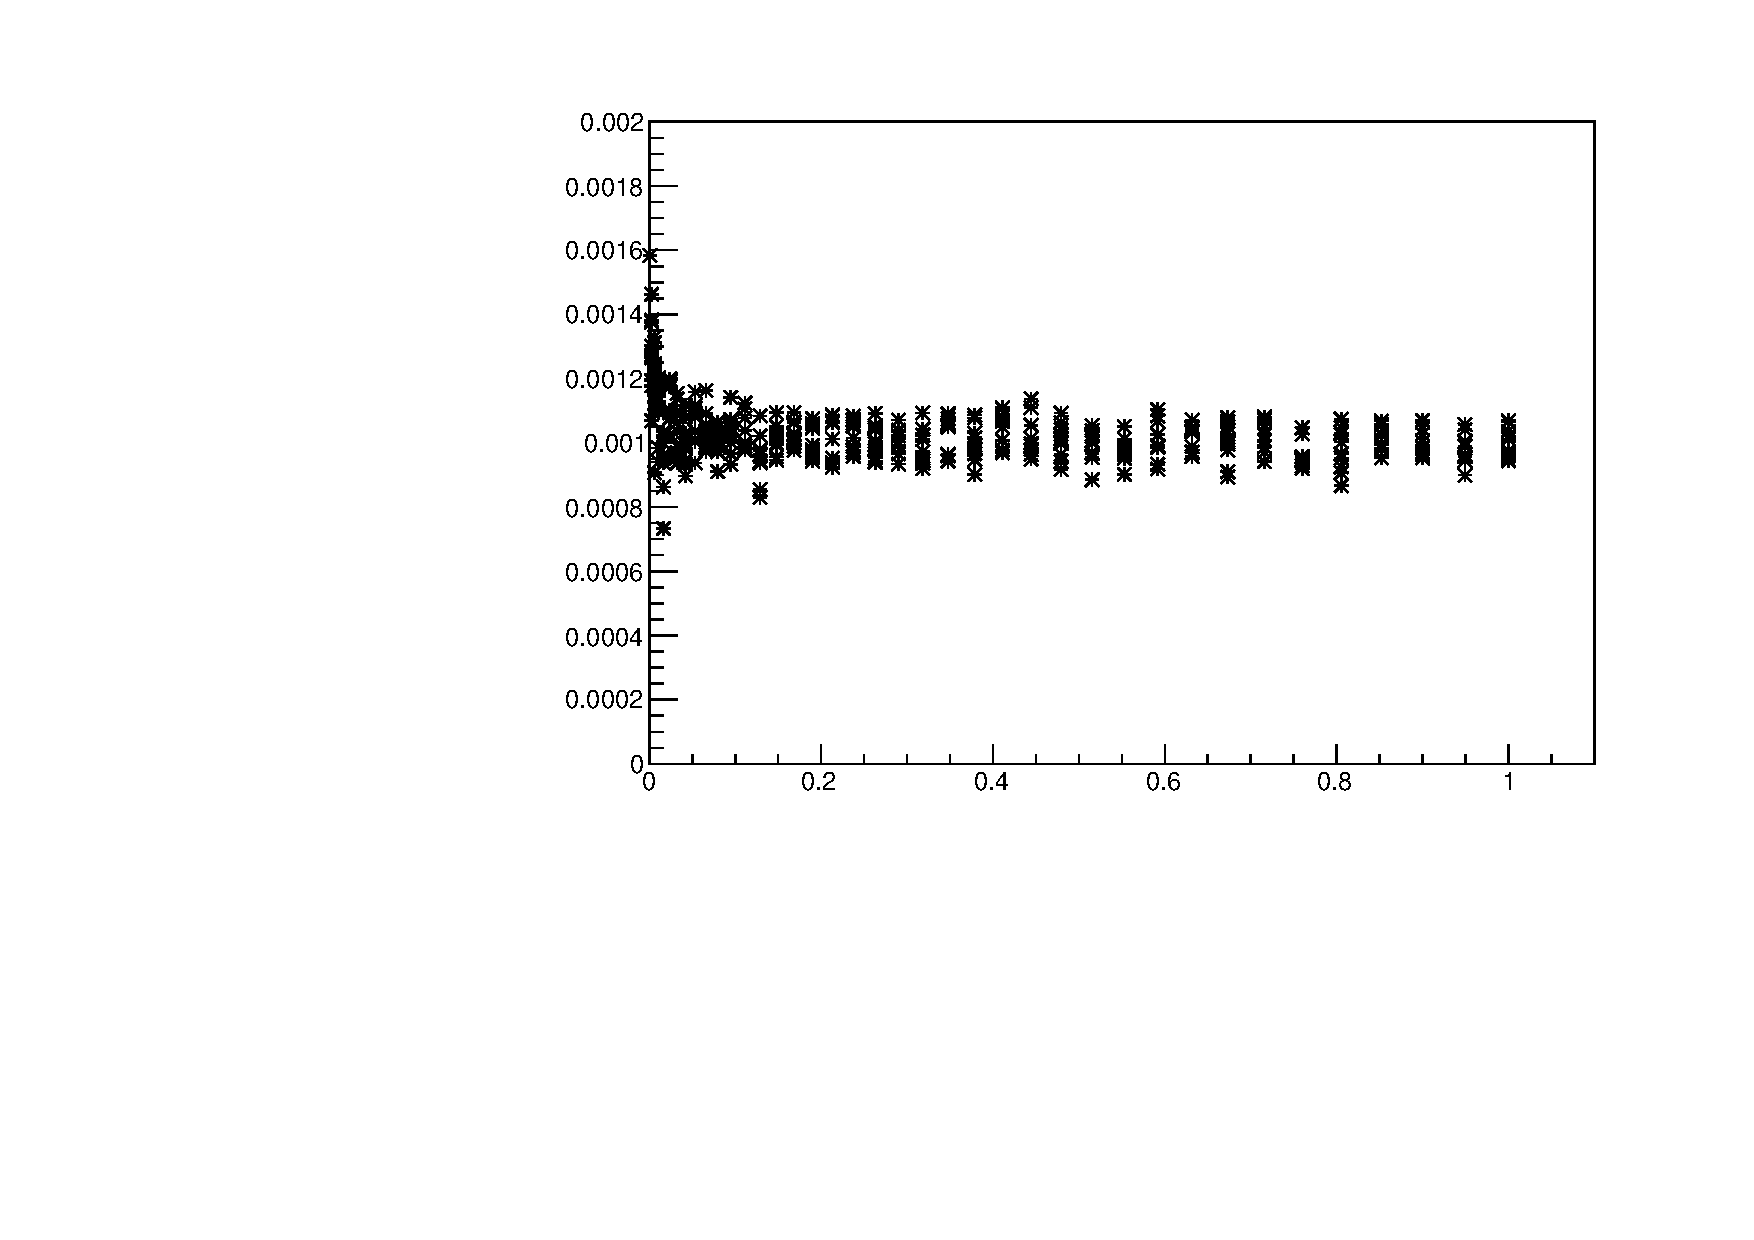
\includegraphics[width=.7\textwidth]{fig/bunny_globmed.pdf}
\caption{random translation of $0.01$ and rotation of $15 \si{\degree}$, chosen $10$ times}
\label{fig:bunny_globmed}
\end{figure}

\begin{figure}[H]
\centering
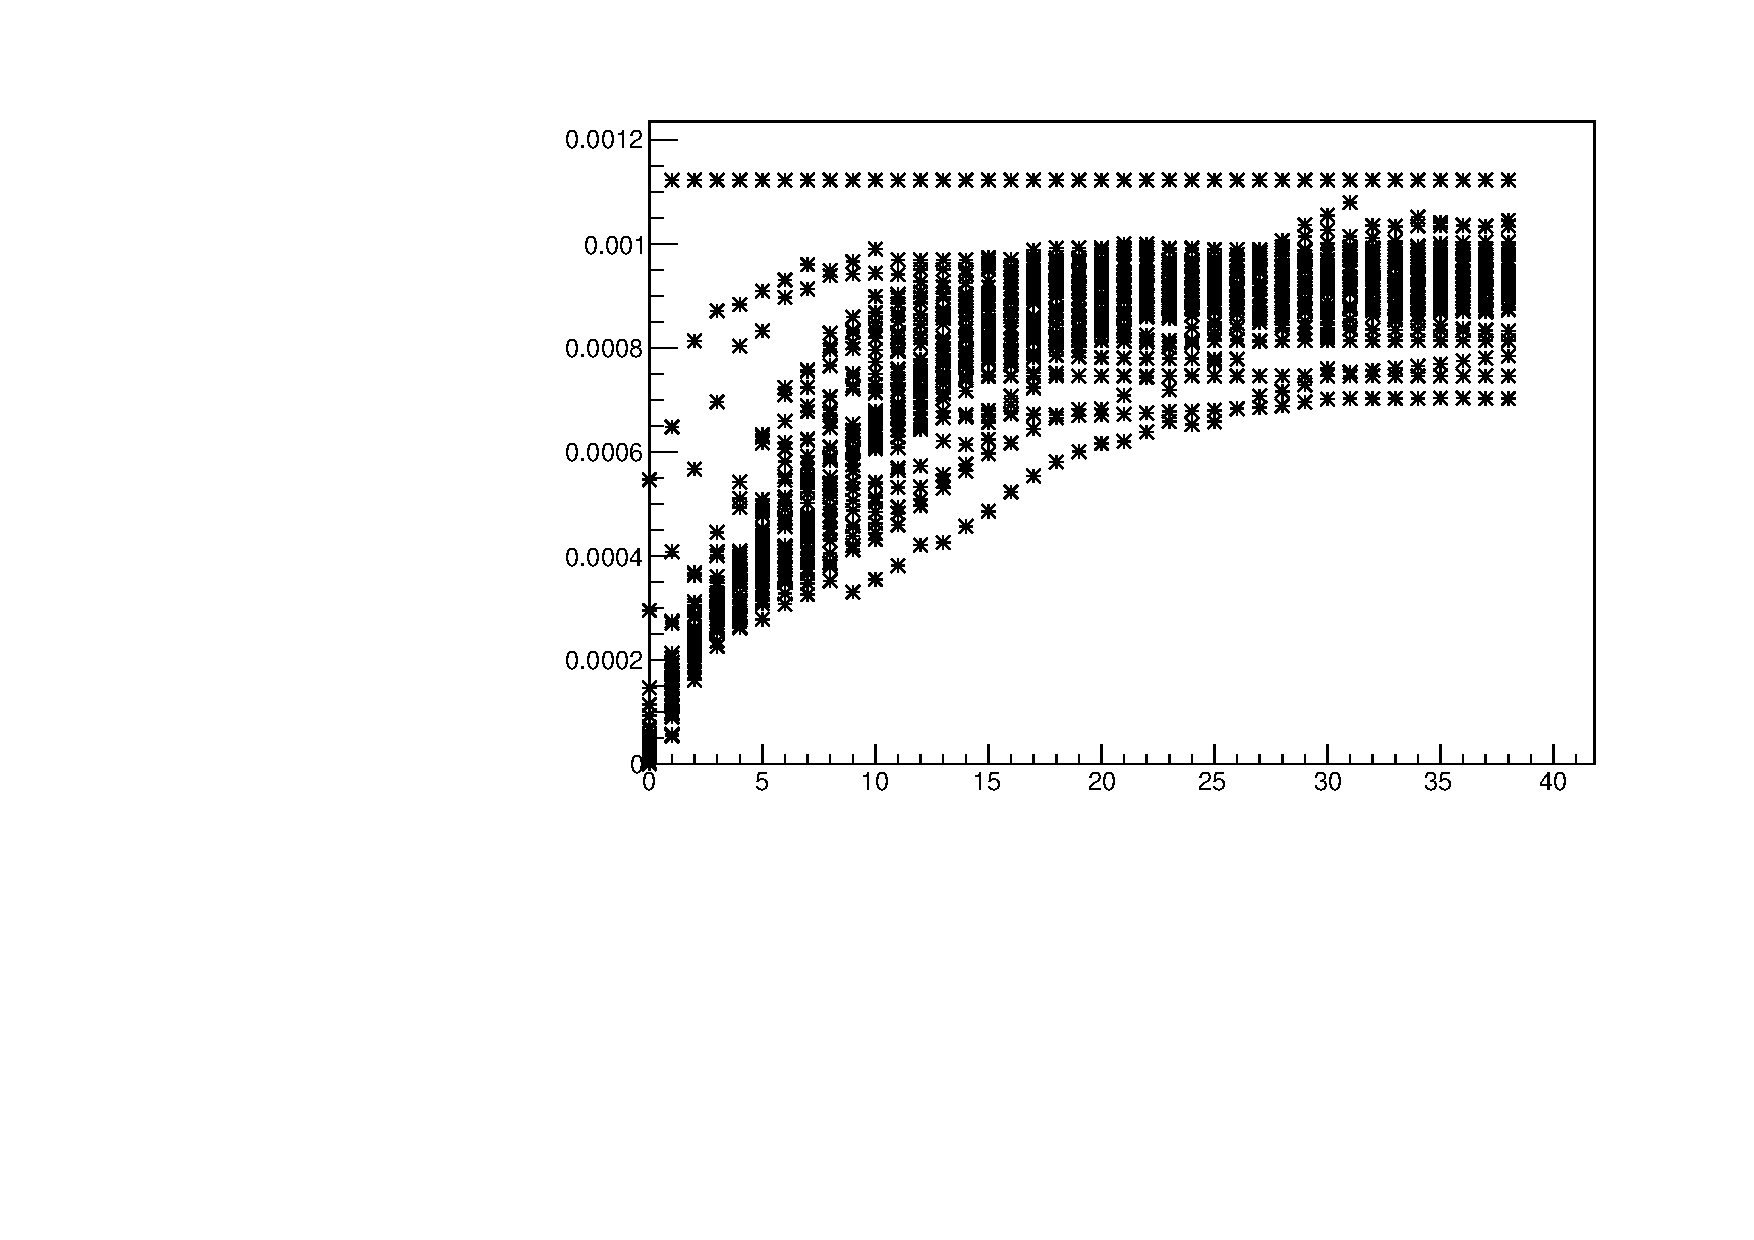
\includegraphics[width=.7\textwidth]{fig/bunny_globmin_ev.pdf}
\caption{Evolutions of true error for experiment \ref{ref:bunny_hilo_a}}
\label{ref:bunny_hilo_ev}
\end{figure}
